\subsection{Component-Bus-System-Property (CBSP) (JEM)}\label{cbsp}
Component-Bus-System-Property, kurz CBSP, ist ein leichtgewichtiger Ansatz, um Anforderungen und Architektur mit Hilfe von Zwischenmodellen in \"Ubereinstimmung zu bringen \cite{Gru01}. Dazu wird iterativ aus den Anforderungen ein CBSP-Modell gebildet, welches Anforderungs- und Architektur-Modellelemente miteinander verkn\"upft. \\

\subsubsection{Ziele der Methode}

Der CBSP-Ansatz hilft Software-Architekten dabei, Architekturelemente wie Komponenten und Konnektoren, Architektur-Eigenschaften, Abh\"angigkeiten zwischen diesen Elementen und passende Architekturstile zu finden. Dabei unterst\"utzt das CBSP den Software-Architekten dabei folgende Herausforderungen, um Anforderungen und Architektur in \"Ubereinstimmung zu bringen, zu behandeln: \\

\begin{itemize}
\item \textit{\"Uberbr\"uckung unterschiedlicher Formalit\"atsebenen}: Das Zwischenmodell von CBSP reduziert die semantische L\"ucke zwischen meist informell in nat\"urlicher Sprache gehaltenen Anforderungen auf einer h\"oheren Abstraktionsebene und eher formell gehaltenen Architekturbeschreibungen \cite{Gru01}.
\item \textit{Modellierung nicht-funktionaler Anforderungen}: CBSP erm\"oglicht, die sonst schwere Modellierung von nicht-funktionalen Anforderungen als Architekturmodell sowohl auf der System- wie auch der Architekturebene \cite{Gru01}. 
\item \textit{Aufrechterhaltung evolution\"arer Konsistenz}: Aufrechterhaltung von Konsistenz und Nachverfolgbarkeit ist ein schwieriges Unterfangen, da eine einzelne Anforderung mehrere architektonische Anliegen betreffen kann und ein einzelnes Architekturelement typischerweise mehrere Beziehungen zu verschiedenen Anforderungen hat \cite{Gru01}. Diese Schwierigkeiten werden vom CBSP-Zwischenmodell behoben.
\item \textit{Unvollst\"andige Modelle und iterative Entwicklung}: Das CBSP-Zwischenmodell ben\"otigt auf Grund seines iterativen Vorgehensmodells keine von Beginn an vollst\"andige Anforderungsspezifikation. Desweiteren k\"onnen bestimmte Anforderungen erst vollst\"andig verstanden werden, wenn die Software-Architektur modelliert oder sogar partiell implementiert wurde \cite{Gru01}.
\item \textit{Gr\"o\ss{}e und Komplexit\"at behandeln}: Gro\ss{}systeme m\"ussen meist hunderte bis tausende von Anforderungen erf\"ullen. Da CBSP sich in jeder Iteration nur mit einem Teil der architektonisch relevanten Anforderungen besch\"aftigt, kann es diese Komplexit\"at beherrschen und den Fokus erh\"ohen. Jede Aktivit\"at von CBSP befasst sich mit der Filterung von Anforderungen oder dem Zusammenfassen mehrerer Anforderungen in eine \cite{Gru01}.
\item \textit{Verschiedene Stakeholder mit unterschiedlichen Interessen}: Anforderungen und Architektur in Einklang zu bringen ist auch ein Prozess, in welchem heterogene Stakeholder mit widerspr\"uchlichen Zielen, Erwartungen und Terminologien involviert sind. CBSP versucht hier die richtige Balance zwischen diesen abweichenden Interessen zu finden, indem es wichtige Stakeholder involviert \cite{Gru01}. \\
\end{itemize}

Um bei der Bew\"altigung dieser Herausforderungen zu unterst\"utzen bietet das CBSP: \\

\begin{itemize}
\item einen leichtgewichtigen Ansatz Anforderungen zu verfeinern durch die Bereitstellung eines kleinen erweiterbaren Sets von Architektur-Schl\"usselkomponenten, 
\item einen Mechanismus um die Anzahl relevanter Anforderungen zu reduzieren und auf die relevantesten ASFRs zu fokussieren, 
\item Beteiligung von wichtigen Stakeholdern, 
\item einen regulierbaren Voting-Mechanismus um Konflikte und unterschiedliche Auffassungen zwischen Architekten zu beheben und
\item Toolunterst\"utzung f\"ur bestimmte Schritte des Ansatzes \cite{Gru01}. \\
\end{itemize}

\subsubsection{Funktionsweise der Methode}

Das CBSP erweitert, wie in Abbildung \ref{fig_cbsp_model} zu sehen ist, den Gedanken des Twin-Peaks Modells. Das Zwischenmodell des CBSP verkn\"upft die Anforderungen mit der Architektur. Das iterative Vorgehen kann dabei sogar auf verschiedenen Detail- bzw. Abstraktionsstufen angewandt werden \cite{Gru01}. 
Um das Vorgehen genauer verstehen zu k\"onnen wird zun\"achst die Taxonomie des CBSP betrachtet. \\

\begin{figure}[h]
	\centering
	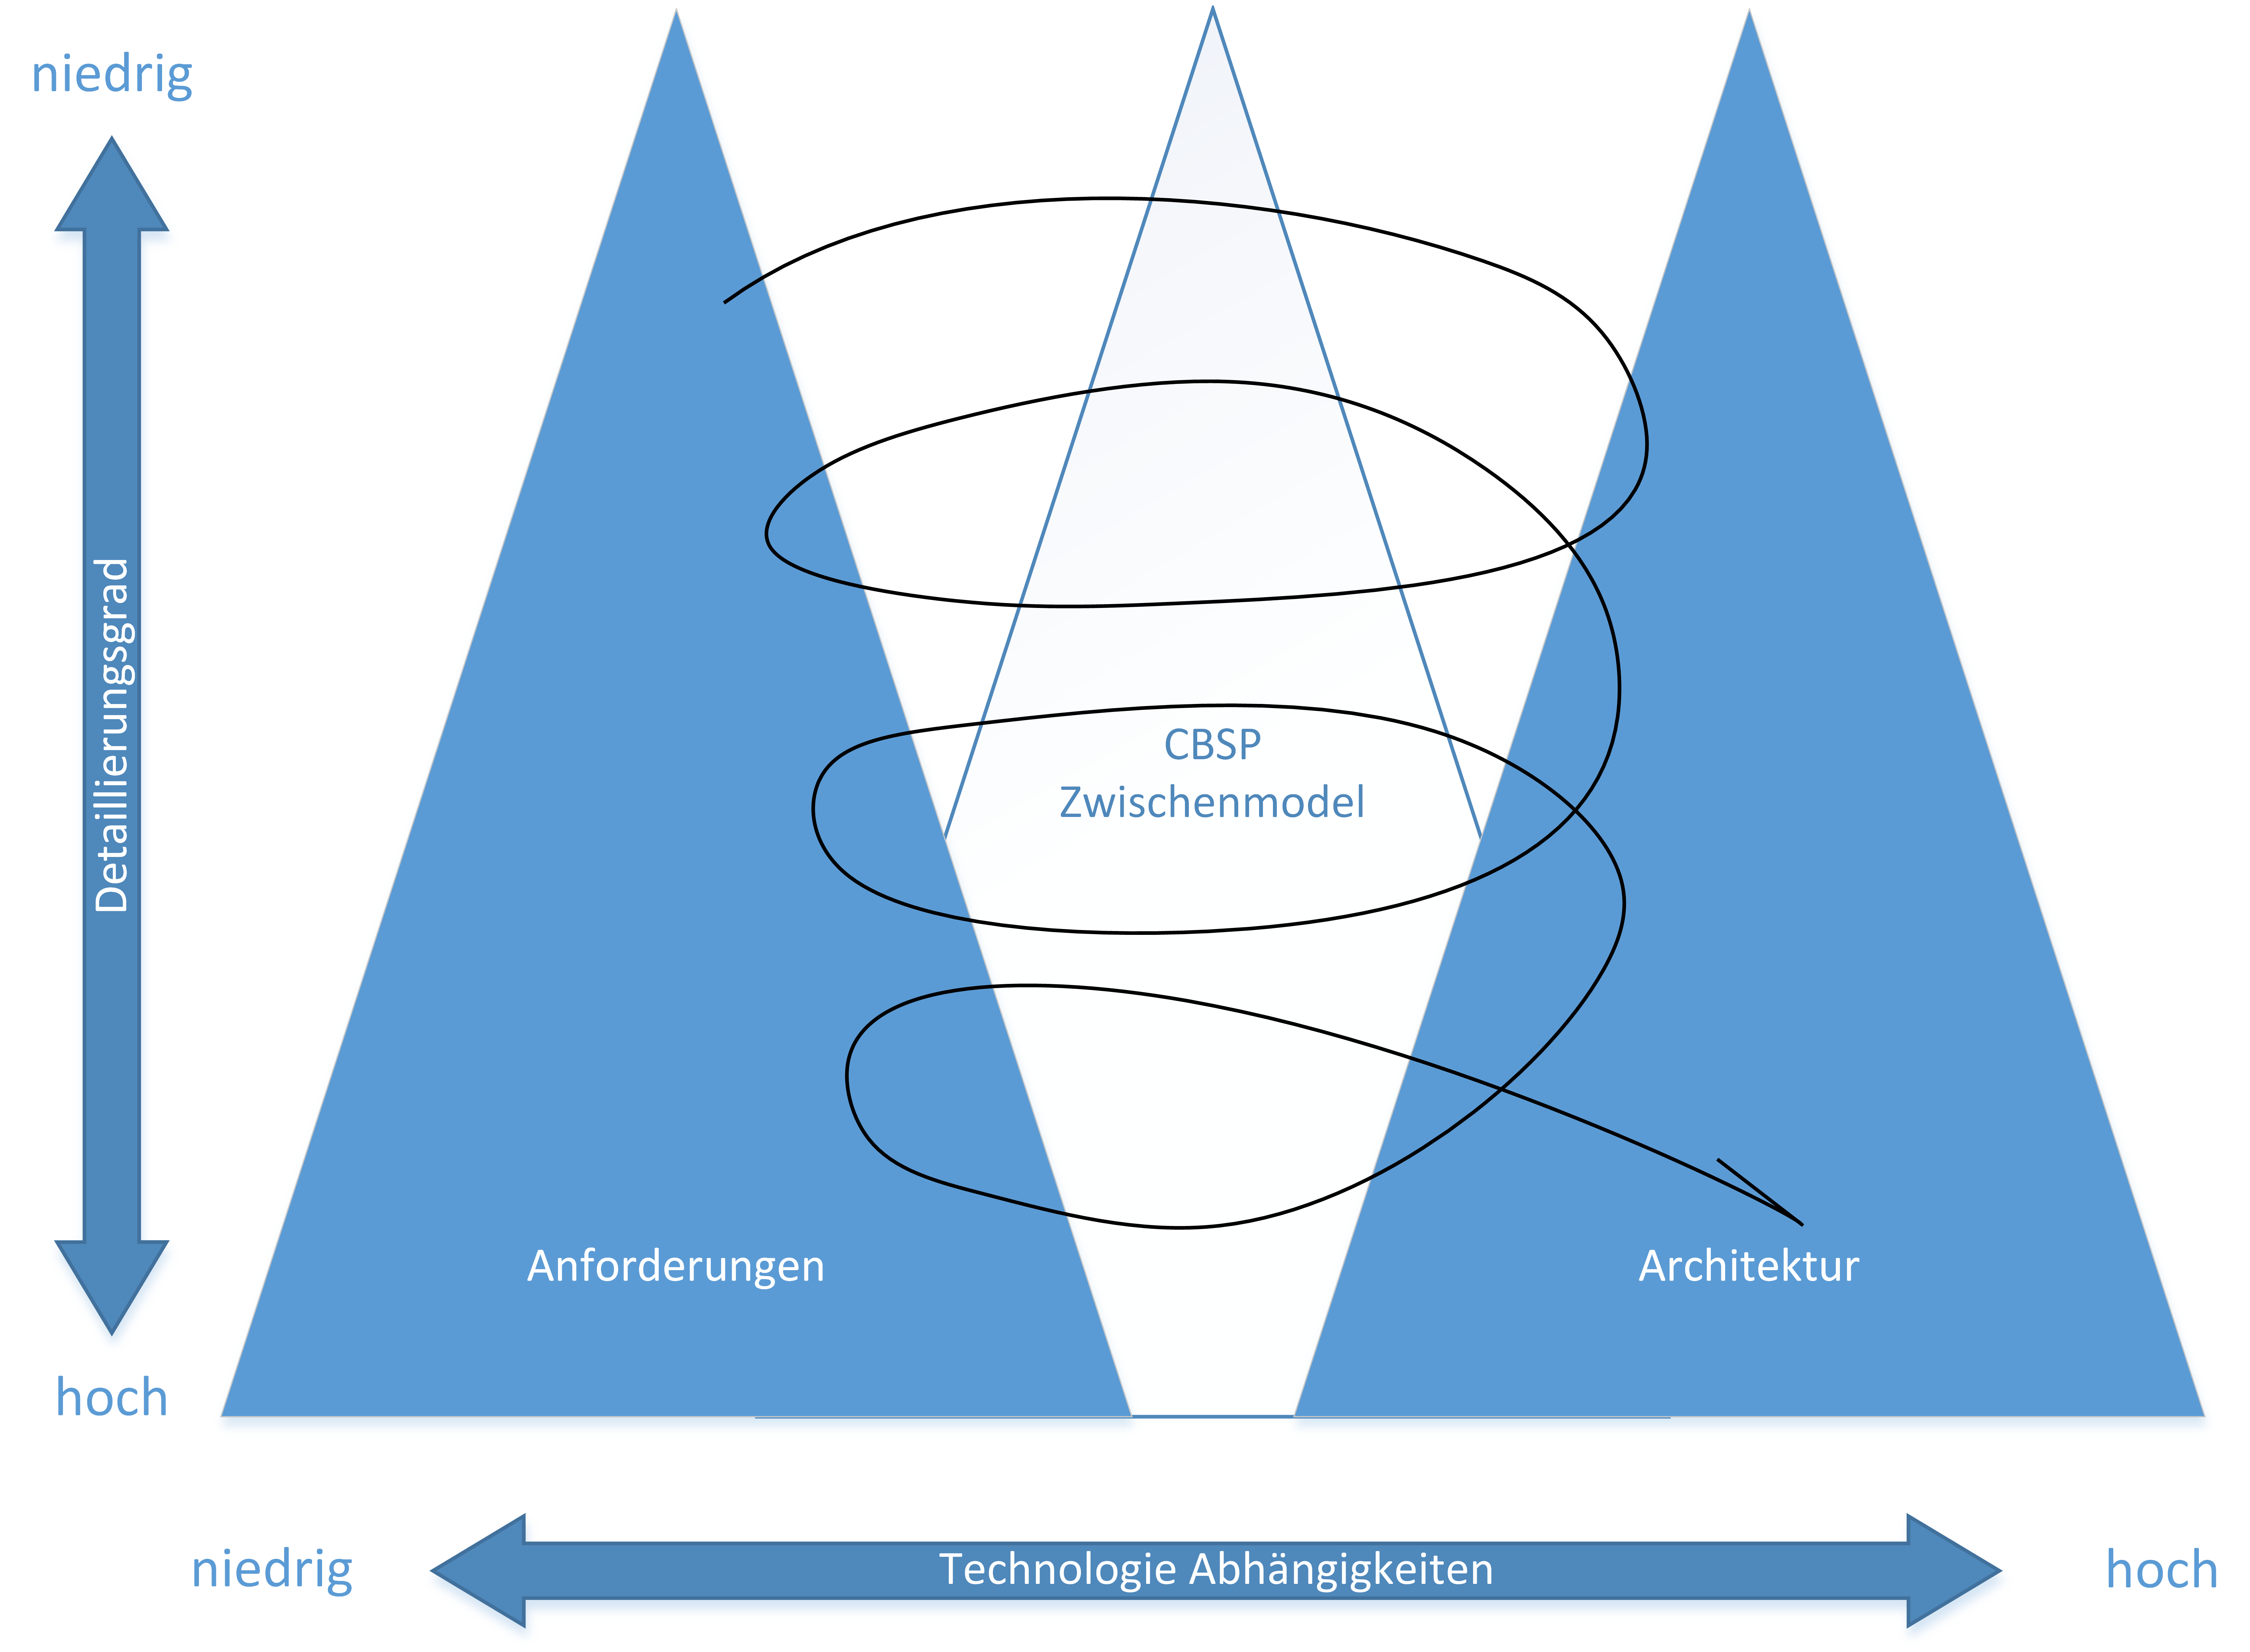
\includegraphics[scale=0.5]{cbsp_model2.png} 
	\caption{CBSP Modell Kontext \cite{Gru01}}
	\label{fig_cbsp_model}
\end{figure}

\emph{CBSP Taxonomie:}
Das Metamodell von CBSP beinhaltet die Basiskonstrukte einer Architektur und ist in sechs Dimensionen aufgeteilt: \\

\begin{itemize}
\item[1.] \textit{C}: sind Elemente, welche individuelle Komponenten der Software-Architektur beschreiben oder involvieren. Diese sind in Datenkomponenten (C\textsubscript{D}) und Verarbeitungskomponenten (C\textsubscript{P}) unterteilt. So k\"onnte beispielsweise die Anforderung: \\
	\textit{R: Benutzern das direkte manipulieren von Kalkulationstabellen erlauben.} \\
	in folgende CBSP Modellelemente verfeinert werden: \\
	\textit{C\textsubscript{P}: UI Komponente f\"ur Kalkulationstabellen Manipulation.} \\
	\textit{C\textsubscript{D}: Daten f\"ur Kalkulationstabellen.}  \cite{Gru01}
\item[2.] \textit{B}: sind Elemente, welche Konnektoren beschreiben. Zum Beispiel: \\
	\textit{R: Manipulierte Daten in Kalkulationstabellen müssen im Dateisystem gespeichert werden.} \\
	kann in folgendes CBSP Modellelement verfeinert werden: \\
	\textit{B: Konnektor, der die Interaktion zwischen UI und Persistenz-Komponenten erm\"oglicht.} \cite{Gru01}
\item[3.] \textit{S}: sind Elemente, welche systemweite Features beschreiben oder solche, die zu einer gr\"o\ss{}eren Untermenge von Komponenten und Konnektoren passen. Zum Beispiel: \\
	\textit{R: Der Benutzer soll angemessene Filter und Visualisierungen ausw\"ahlen k\"onnen.} \\
	kann in folgendes CBSP Modellelement verfeinert werden: \\
	\textit{S: Das System soll eine strikte Trennung von Datenhaltungs-, -Bearbeitungs- und -Visualisierungs-Komponenten vornehmen.} \cite{Gru01}
\item[4.] \textit{CP}: sind Elemente, welche Eigenschaften, wie Zuverl\"assigkeit, Portabilit\"at, Skalierbarkeit, Anpassbarkeit und Erweiterbarkeit, von Daten- oder Verarbeitungskomponenten beschreiben. Zum Beispiel: \\
	\textit{R: Der Benutzer soll die Daten entfernt mit minimale wahrgenommener Latenz visualisieren k\"onnen.} \\
	kann in folgendes CBSP Modellelement verfeinert werden: \\
	\textit{CP: Die Datenvisualisierungs-Komponente soll effizient sein und inkrementelle Updates unterst\"utzen.} \cite{Gru01}
\item[5.] \textit{BP}: sind Elemente, welche Eigenschaften von Konnektoren beschreiben. Zum Beispiel: \\
	\textit{R: Updates f\"ur Systemfunktionen sollen mit minimaler Ausfallzeit m\"oglich sein.} \\
	kann in folgendes CBSP Modellelement verfeinert werden: \\
	\textit{BP: Robuste Konnektoren sollen zur Verf\"ugung gestellt werden, um das Hinzuf\"ugen und Entfernen von Laufzeitkomponenten zu erleichtern.} \cite{Gru01}
\item[6.] \textit{SP}: sind Elemente, welche systemweite Eigenschaften bzw. Eigenschaften von Subsystemen beschreiben. Zum Beispiel: \\
	\textit{R: Die Daten der Kalkulationstabellen m\"ussen verschl\"usselt werden, bevor sie \"uber das Netzwerk versandt werden.} \\
	kann in folgendes CBSP Modellelement verfeinert werden: \\
	\textit{SP: Das System soll sicher sein.} \cite{Gru01} \\
\end{itemize}

Aus diesen Elementen wird das CBSP Zwischenmodell aufgebaut. Das Metamodell zu diesen Elementen ist in Abbildung \ref{fig_cbsp_meta_model} dargestellt. Jedes CBSP Artefakt beschreibt ein architekturrelevantes Anliegen und beschreibt eine fr\"uhe Architekturentscheidung des zu erstellenden Systems \cite{Gru01}. \\

Von einer Anforderung zu einem CBSP Element kann eine Verfeinerung, siehe Beispiel (5), oder Generalisierung, siehe Beispiel (6), erfolgen. Diese beiden m\"oglichen Anpassungen basieren auf Notwendigkeiten, welche durch bestimmte Eigenschaften des zu erstellenden Systems, Charakteristika der Anwendungsdom\"ane oder Hintergrund und Erfahrung des Software-Architekten, erwachsen \cite{Gru01}. Da es f\"ur Verfeinerung und Generalisierung keine allgemeinen formalen Regeln gibt, ist es h\"aufig notwendig, hierf\"ur den Kunden bzw. weitere Stakeholder wie den Requirements Engineer zu konsultieren \cite{Gru01}. 

\begin{figure}[h]
	\centering
	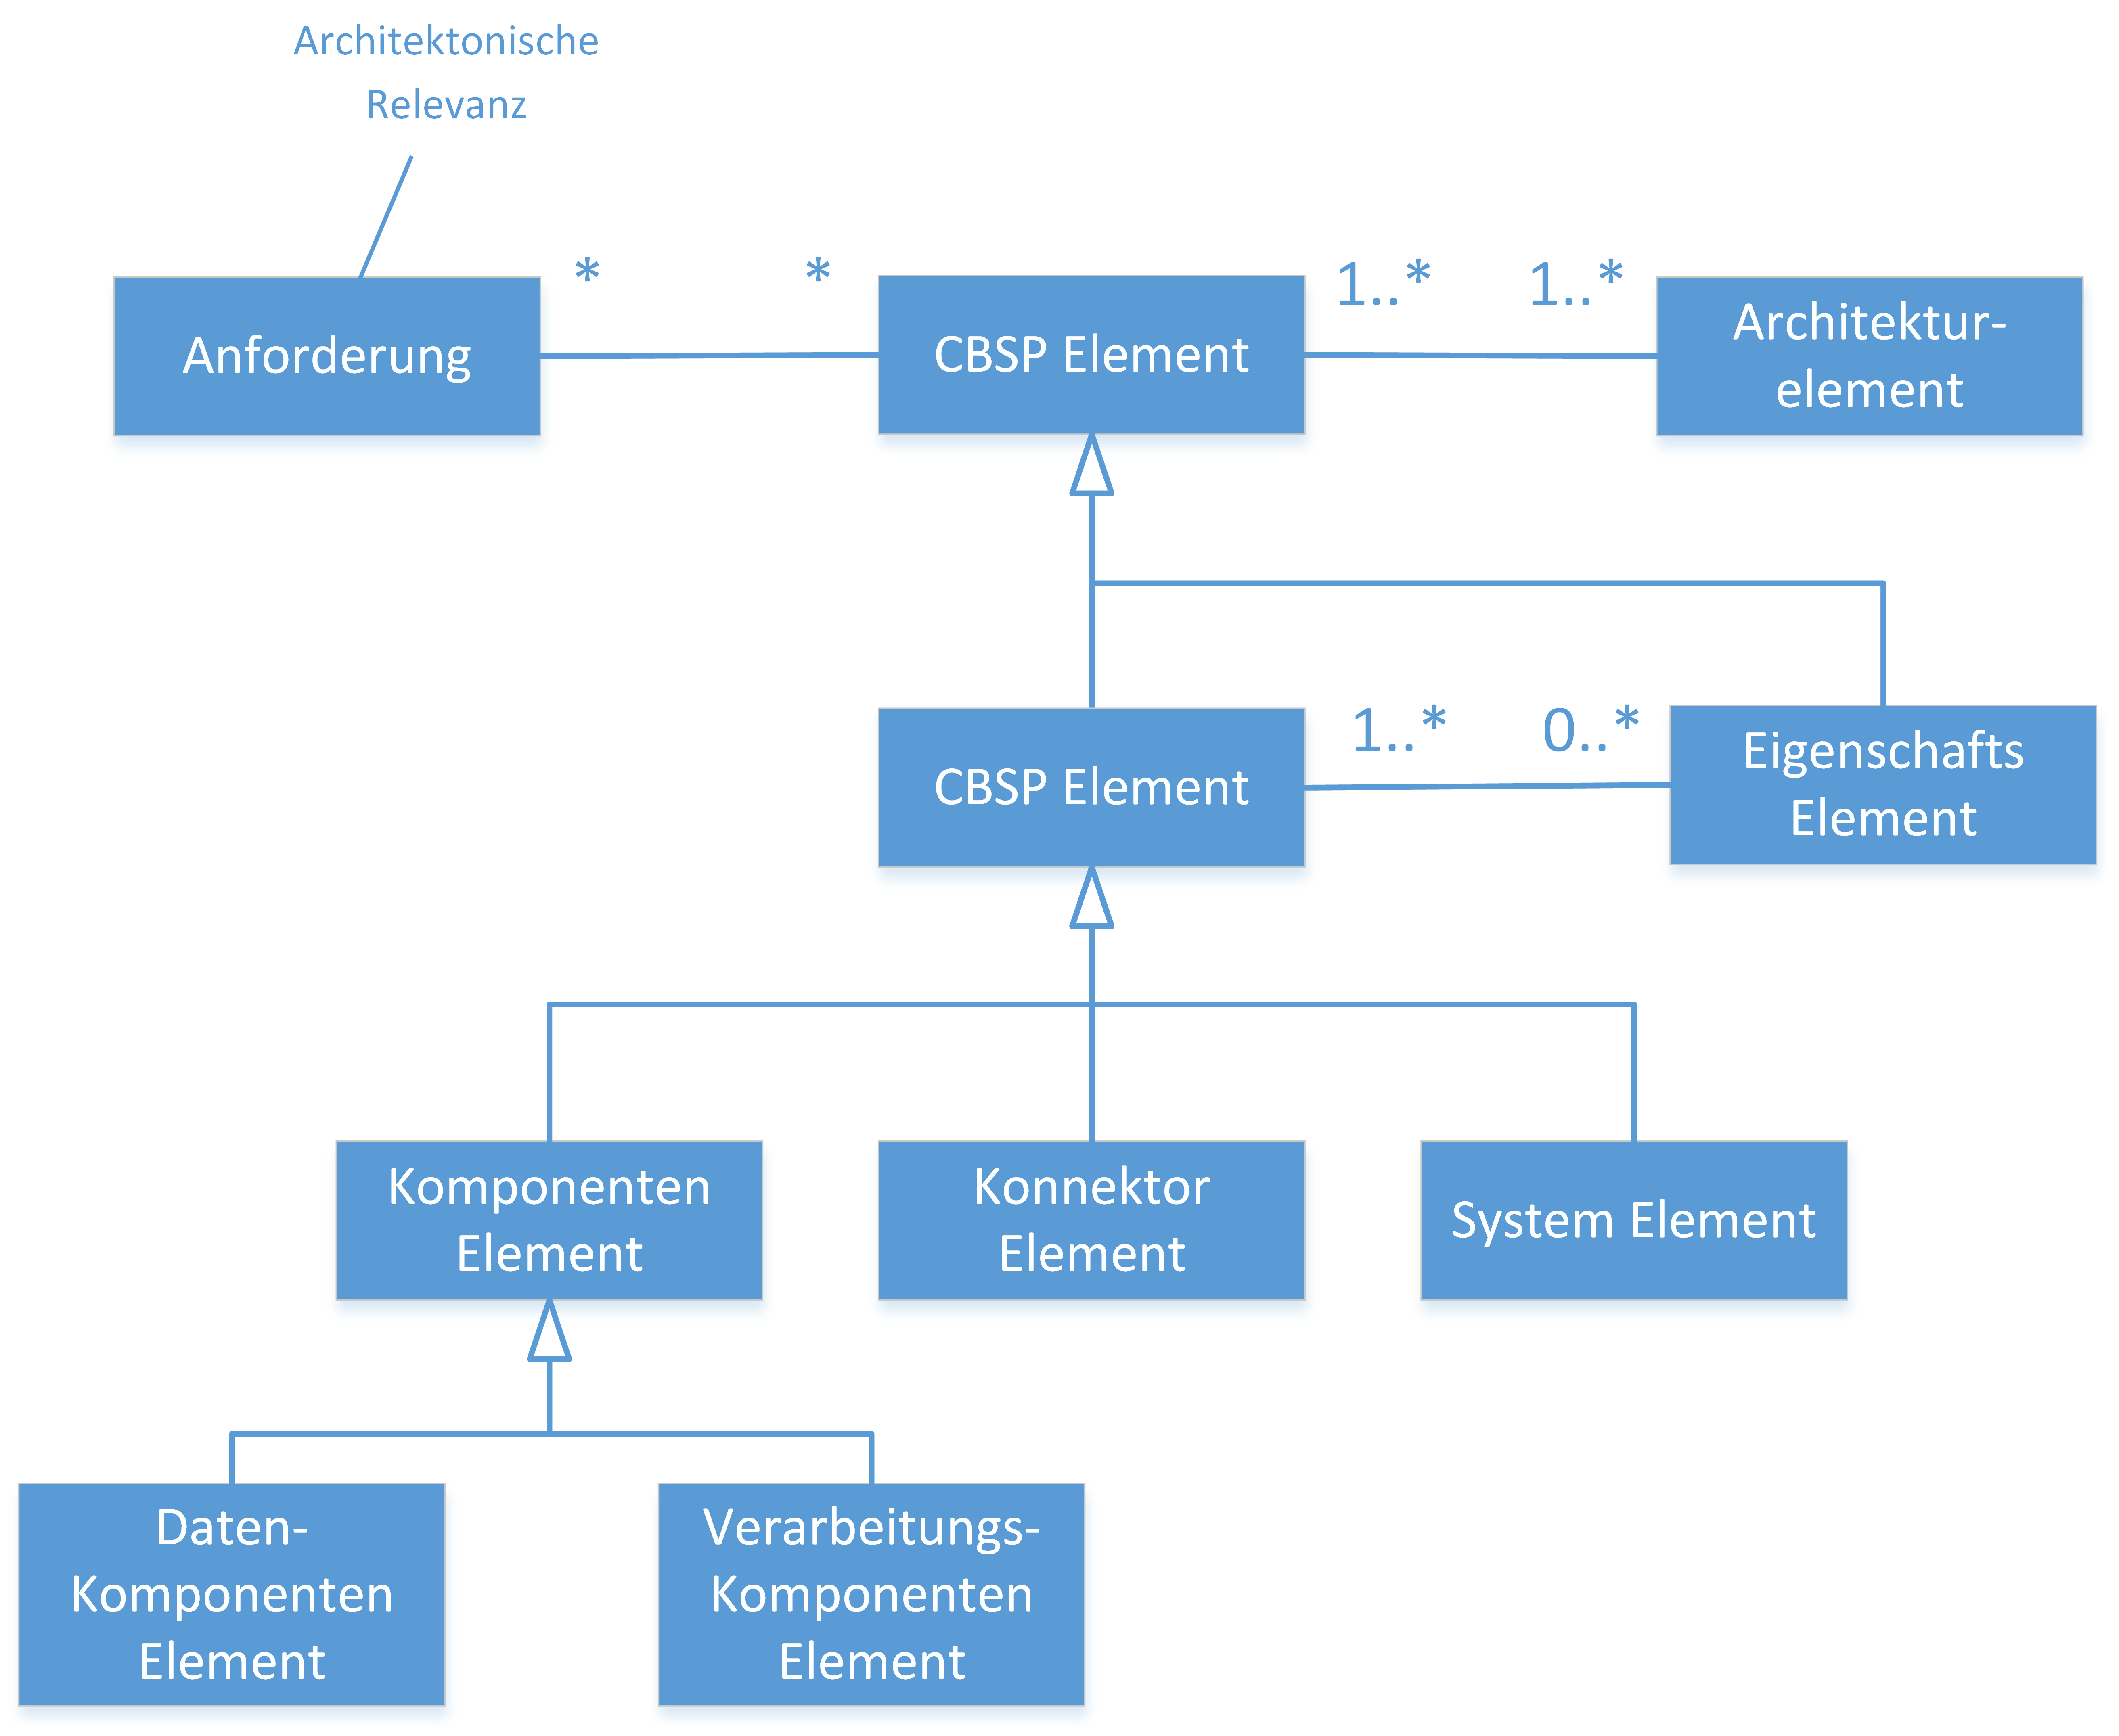
\includegraphics[scale=0.6]{cbsp_meta_model.png} 
	\caption{CBSP Metamodell \cite{Gru01}}
	\label{fig_cbsp_meta_model}
\end{figure}

\paragraph{Randbedingungen}

Damit CBSP erfolgreich angewandt werden kann, muss die Bereitschaft zur Mitarbeit aller involvierten Stakeholder gegeben sein. In fast allen Schritten k\"onnen diese bei Unklarheiten oder f\"ur Feedback herangezogen werden. In einigen Schritten ist deren Mitarbeit verpflichtend. \\
Des Weiteren m\"ussen die Software-Architekten \"uber ein gewisses Mindestma\ss{} an Erfahrung und Wissen verf\"ugen um die einzelnen Schritte kompetent durchf\"uhren zu k\"onnen. Daf\"ur gibt es allerdings keine Liste mit Mindestvoraussetzungen oder ein Minimum an Jahren an Berufserfahrung. Hier muss klar sein, ob der Architekt die n\"otigen Kompetenzen besitzt um wichtige Entscheidungen selbstst\"andig treffen zu k\"onnen. \\

\paragraph{Eingabe}

Als Eingabe ben\"otigt das CBSP eine erste Anforderungsspezifikation. Diese muss noch nicht vollst\"andig sein, denn sie kann in jeder Iteration weiter erg\"anzt werden. Da CBSP nicht auf FRs oder NFRs zugeschnitten ist, werden alle Anforderungen genutzt, denn beide Anforderungstypen haben sowohl explizit als auch implizit Informationen, welche f\"ur die Software-Architektur relevant sind \cite{Gru01}. \\


\paragraph{Vorgehensmodell} 
Jede Iteration von CBSP besteht aus f\"unf Schritten, welche im folgenden vorgestellt werden. \\

\emph{Schritt 1: Auswahl der Anforderungen f\"ur die n\"achste Iteration} - 
Um die Komplexit\"at zu reduzieren werden hier, wie bereits angesprochen, durch ein Team von Architekten nur Anforderungen f\"ur die Iteration ausgew\"ahlt, welche mittels zweier Kriterien durch den Requirements Engineer als wichtig oder durchf\"uhrbar bewertet wurden: (1) die \textit{Bedeutung} zeigt die Relevanz und den Wert f\"ur den Projekterfolg, (2) w\"ahrend die \textit{Durchf\"uhrbarkeit} technische, \"okonomische und politische Bedingungen ber\"ucksichtigt \cite{Gru01}. Diese Anforderungen k\"onnen formell, informell oder semi-formell notiert sein. \\

\emph{Schritt 2: Architektonische Klassifizierung der Anforderungen} - 
In Schritt zwei klassifizieren die Software-Architekten die selektierten Anforderungen mit Hilfe der CBSP Taxonomie. Desweiteren werden alle so klassifizierten Anforderungen in einer Tabelle anhand ihrer Relevanz zu den sechs CBSP Dimensionen bewertet. Die Bewertung erfolgt \"uber eine Ordinalskala (nicht=0; partiell=1; weitgehend=2; voll=3) und beschreibt die Auswirkung, welche die Anforderung auf eine oder mehrere der jeweiligen CBSP Elemente hat \cite{Gru01}. Eine beispielhafte Bewertung der Anforderungen \textit{R01: Unterschiedliche Ladungstypen unterst\"utzen}, \textit{R02: Verschiedene Fahrzeuge unterst\"utzen} und \textit{R09: Sch\"atzung der Frachtankunft und Fahrzeugverf\"ugbarkeit unterst\"utzen} ist Tabelle \ref{tab:relevance_profiles} zu entnehmen \cite{Gru01}. 

\begin{table}[h] %h, t, b, p : here = genau an dieser Stelle, wenn m\"oglich, top = f\"ur den Seitenanfang, bottom = f\"ur das Seitenende, p = f\"ur eine spezielle Seite mit Tabellen und Abbildungen
\caption{Beispiel Relevanzprofile nach \cite{Gru01}}
\centering
\begin{tabular}{|l|c|c|c|c|c|c|}
\hline 
\textbf{Anforderungen} & \textbf{C} & \textbf{B} & \textbf{S} & \textbf{CP} & \textbf{BP} & \textbf{SP} \\ 
\hline 
R01 & 1,33 & 0,33 & \cellcolor{Gray} 1,67 & 1,00 & 0,33 & 0,33 \\ 
\hline 
R02 & \cellcolor{Gray} 2,00 & 0,00 & 1,00 & 1,33 & 0,00 & 0,00 \\ 
\hline 
R09 & \cellcolor{Gray} 2,67 & 1,33 & 2,00 & 0,33 & 0,00 & 0,00 \\ 
\hline 
\end{tabular} 
\label{tab:relevance_profiles}
\end{table}

\begin{table*}[t] %h, t, b, p : here = genau an dieser Stelle, wenn m\"oglich, top = f\"ur den Seitenanfang, bottom = f\"ur das Seitenende, p = f\"ur eine spezielle Seite mit Tabellen und Abbildungen
\caption{CBSP zu Architekturstil Mapping nach \cite{Gru01}}
\centering
\newcolumntype{M}[1]{>{\centering\arraybackslash}p{#1cm}}
\begin{tabular}{|p{3cm}|p{4,2cm}|M{2}|M{1}|M{2}|M{1,5}|M{1,3}|}%{|l|c|c|c|c|c|c|} 15
\hline 
\textbf{CBSP Dimensionen} & \textbf{Eigenschaften} & \textbf{Client-Server} & \textbf{C2} & \textbf{Event-basiert} & \textbf{Schichten-Architektur} & \textbf{Pipes und Filter} \\ 
\hline 
Datenkomponente & aggregiert & ++ & ++ & ++ & + & - \\ 
 & persistent & ++ & o & o & o & o \\ 
 & gestreamt & - & - & - & - & + \\ 
 & gecached & ++ & + & - & - & - \\ 
\hline 
Verarbeitungskomponente & Dienste anbieten / Nur konsumieren & ++ & o & o & o & o \\ 
 & hat N Schnittstellen & ++ & + & ++ & - & - \\ 
 & stateful & + & ++ & ++ & + & - \\ 
 & lose gekoppelt & + & + & ++ & - & ++ \\ 
 & kann migriert werden & + & ++ & ++ & - & - \\ 
\hline 
Konnektor & synchron & ++ & - & + & ++ & - \\ 
 & asynchron & - & ++ & ++ & - & ++ \\ 
 & lokal & - & ++ & o & ++ & + \\ 
 & verteilt & ++ & ++ & ++ & - & + \\ 
 & sicher & + & o & o & + & o \\ 
\hline 
(Sub-)System & effizient & o & + & + & o & - \\ 
 & skalierbar & + & o & - & - & + \\ 
 & weiterentwickelbar & ++ & ++ & ++ & - & ++ \\ 
 & portierbar & o & + & o & ++ & o \\ 
 & zuverl\"assig & o & o & - & o & o \\ 
 & dynamisch & + & ++ & ++ & - & ++ \\
\hline 
\end{tabular} 
\label{tab:cbsp_to_style_mapping}
\end{table*}

\emph{Schritt 3: Identifizierung und Aufl\"osung von falschen Zuordnungen bei der Klassifizierung} - 
Da mehrere Software-Architekten diese Klassifizierung unabh\"angig voneinander vornehmen, m\"ussen im dritten Schritt m\"ogliche Abweichungen aufgedeckt, diskutiert und behoben werden. Dies ist wichtig um Missverst\"andnisse, mehrdeutige Anforderungen, implizites Wissen, und widerspr\"uchliche Auffassungen zu identifizieren und Risiken bei der Verfeinerung der Anforderungen zu reduzieren \cite{Gru01}. Bei der Diskussion k\"onnen auch der Kunde und Requirements Engineer involviert sein. Der erarbeitete Konsens sorgt f\"ur ein einheitliches Verst\"andnis der Anforderungen und die Relevanz dieser f\"ur die Software-Architektur. Wenn keine Unstimmigkeiten mehr vorliegen, werden die Anforderungen weiter ausged\"unnt indem alle Anforderungen, welche eine geringere Relevanz haben als ein vorher definierter Wert der Ordinalskala, wie beispielsweise "weitgehend", vorerst verworfen werden. Dabei wird auf Abh\"angigkeiten zwischen den Anforderungen geachtet um kritische nicht zu verwerfen. Alle akzeptierten Anforderungen werden inklusive gesammelter Probleme und Unklarheiten in den n\"achsten Schritt \"ubernommen. \\

\emph{Schritt 4: Architektonische Verfeinerung der Anforderungen} - 
Im vorletzten Schritt werden die CBSP Elemente umformuliert oder aufgeteilt, welche \"uberlappende CBSP Dimensionen und architektonische Anliegen aufweisen. Wenn ein CBSP Element beispielsweise weitgehend Komponenten-relevant, voll Konnektor-relevant und weitgehend Konnektor-Eigenschafts-relevant ist, erh\"oht es das Verst\"andnis und die Pr\"azision, wenn es in mehrere Architekturentscheidungen, verk\"orpert als CBSP Element, aufgesplittet wird. Ein einzelnes CBSP Artefakt kann w\"ahrend dieses Prozesses mehrfach als Nebenprodukt bei verschiedenen Anforderungen auftauchen, w\"ahrend diese Redundanzen identifiziert und eliminiert werden \cite{Gru01}. \\

In diesem Schritt gibt es zwei Varianten, welche entweder einzeln oder sogar kombiniert ausgef\"uhrt werden k\"onnen. Variante eins betrachtet zun\"achst nur die gro\ss{}en strukturellen Aspekte des Systems (C, B und S Elemente). Dies hat den Vorteil, dass der Architekt leichter einen Überblick behalten kann, da die beiden Aspekte (Struktur und Funktionalit\"at vs. nicht-funktionale Eigenschaften) separat betrachtet werden. Die Eigenschaften der drei Elemente werden in einem gesonderten (Sub-)Prozess identifiziert. Die zweite Variante identifiziert in einem Schritt sowohl die strukturellen Elemente als auch ihre nicht-funktionalen Eigenschaften. Der Vorteil hierbei ist, dass der Software-Architekt sich auf einen einzelnen System-Aspekt (oder eine kleine Menge von Aspekten) konzentrieren kann. \\

\emph{Schritt 5: Abgleich der Entscheidungen zwischen Architekturelementen und -stilen mit CBSP} - 
Wenn alle ausgew\"ahlten Anforderungen im CBSP Model modelliert wurden, sodass keine Konflikte zwischen Software-Architekt und Requirements Engineer bestehen und alle CBSP Modellelemente weitgehend relevant zu einer der sechs CBSP Dimensionen sind, kann in Schritt f\"unf ein erster Architektur-Prototyp abgeleitet werden. \\
Die Bestimmung eines passenden Architekturstiles mit den zu den CBSP Modellelementen passenden Architekturmustern ist nicht immer einfach. Zum einen existiert kein formaler Ansatz f\"ur diesen Prozess, zum anderen k\"onnen mehrere Architekturstile zum generierten CBSP Modell passen. F\"ur diese Aufgabe gibt es verschiedene Verfahren. Hier wird die Selektion eines passenden Architekturstiles mit Hilfe einer Matrix aufgestellt, siehe Tabelle \ref{tab:cbsp_to_style_mapping}. Diese Matrix stellt die CBSP Dimensionen mit geeigneten Eigenschaften potentiellen Architekturmustern gegen\"uber. Allerdings ist diese Tabelle nicht vollst\"andig, denn weitere Eigenschaften f\"ur die CBSP Elemente sind denkbar und es werden auch nicht alle existierenden Architekturstile angeboten. Zum einen ist sie daf\"ur nicht gedacht, sie soll lediglich eine Hilfestellung bei der Wahl eines passenden Architekturstils bieten, sobald mehr als einer passend erscheint. Daf\"ur muss sie nur so umfassend wie eben n\"otig sein. Zum anderen w\"urde eine vollst\"andige Tabelle \textit{jedes} Softwaresystem darstellen und nicht auf eine konkrete Dom\"ane zurecht geschnitten sein. Au\ss{}erdem w\"are eine solche unm\"oglich zu erstellen \cite{Gru01}. Die endg\"ultige Wahl liegt allerdings beim Software-Architekten. \\

Anschlie\ss{}end muss der Software-Architekt die CBSP Modellelemente in entsprechende Architekturelemente wie Komponenten, Konnektoren, Konfigurationen, Pakete und Daten mit den gew\"unschten Eigenschaften umwandeln \cite{Gru01}. \\

\paragraph{Ausgabe}

Nach der Ausf\"uhrung der f\"unf Schritte und mehrfachen Iterationen sollte eine Software-Architektur gegeben sein, welche die selektierten Anforderungen zu einem m\"oglichst hohen Grad erf\"ullt.

%\textbf{Paper Cites:} \\
%(\cite{Gru01}) Reconciling software requirements and architectures with intermediate models \\


%Viel ^^ (Weaving the Software Development Process Between Requirements and Architectures)

%RE und SA sind sehr voneinander abh\"angig (Descending the twin Peaks)


%\begin{itemize}
%\item[1.] Text
%\item[2.] Text
%\item[3.] Text \\
%\end{itemize}